\section{Rat-Like Behavior Interaction}
\subsection{Robotic Rat Platform}
The prototype of our recently developed robotic rat is shown in Figure \ref{figure:robot-system}. The robot is mainly composed of the head, forelimb, waist and hip. The head and hip joints are driven by servo motors, the waist joints and wheels are driven by DC motors, and the forelimb is driven by a micro deceleration stepper motor. Its shape and size are similar to those of actual rats, with a total mass of approximately 400 g. The spinal joints of the robot correspond to the key movement joints of rats. The head pitching and yaw movements ($M_1, M_2$) are performed by $J_7$ and $J_6$ respectively; the body pitching movement $M_3$ is performed by $J_1$, $J_2$ and $J_5$; the body yaw movement ($M_4$) is performed by $J_3$ and $J_4$; the straight movement ($M_5$) is performed by the driving wheels ($J_{WL}$, $J_{WR}$); the turing movement ($M_6$) is performed by the yaw joints compound driving wheels ($J_3$, $J_4$, $J_6$, $J_{WL}$, $J_{WR}$); and the forelimb swing movement ($M_8$) is performed by $J_F$.

\begin{figure}[h]
    \centering
    \begin{subfigure}{0.4\textwidth}
        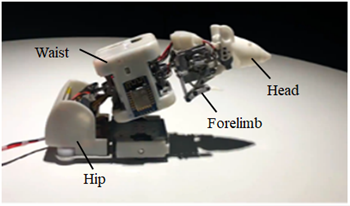
\includegraphics[height=1.3in]{roboticrat.png}
        \caption{\label{figure:roboticrat}}
    \end{subfigure}
    \begin{subfigure}{0.5\textwidth}
        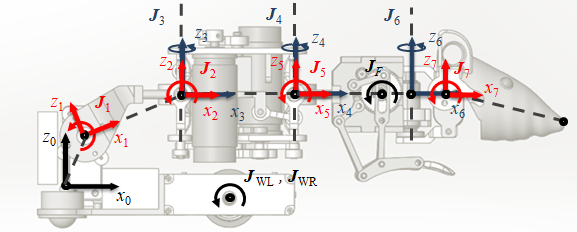
\includegraphics[height=1.3in]{coord.png}
        \caption{\label{figure:motion-coord}}
    \end{subfigure}
    \caption{(\subref{figure:roboticrat}) Robotic rat. (\subref{figure:motion-coord}) Motion coordinate system of the robotic rat.}
    \label{figure:robot-system}
\end{figure}

To make the robot achieve the above behaviors, we extracted the characteristic parameters for each movement combination, as shown in Table \ref{table:Movement Parameters}. These parameters determine the amplitude, average speed, frequency and duration of rat movements. In our previous work, we proved that the robot can complete the movement of rats with a high biomimicry degree, and the trajectory of each joint of the robot can be expressed by the above characteristic parameters \cite{shi-gao-tro-2021}. Here, to adapt to the diversity of rat movement parameters, we first used cluster analysis to extract the dominant values of these characteristic parameters \cite{fraley_how_many_clusters,kaufman_finding_groups}. Furthermore, a two-hidden-layer BP neural network is used to learn and generate the trajectory of each joint of the robot, as shown in Figure. \ref{figure:Joint Trajectory learning by a two hidden-layer BP neural network}. The tanh activation function is used to accelerate the convergence of the network \cite{inohira-generalization}. $\theta_1-theta_7$ represent the angular displacement of robot spine joints, $\theta_f$ represents the angular displacement of robot forelimb joint, and $\omega_l,~\omega_r$ represent the angular velocity of robot driving wheels.

\begin{table}[b]
    \caption{Movement Parameters}
    \centering
    \begin{tabular}{cc}
            \hline
            Movement parameters & Symbol \\
            \hline
            Head pitch angle & $\phi_{hp}$ \\
            Head yaw angle & $\phi_{hy}$ \\
            Body pitch angle & $\phi_{bp}$ \\
            Body yaw angle & $\phi_{by}$ \\
            Forelimb swing angle & $\phi_{fs}$ \\
            Turning angle & $\alpha$ \\
            Average forward speed & $\nu$ \\
            Movement frequency & $f$ \\
            Movement duration & $f$ \\
            \hline
            \end{tabular}
    \label{table:Movement Parameters}
\end{table}

\begin{figure}[h]
    \centering
    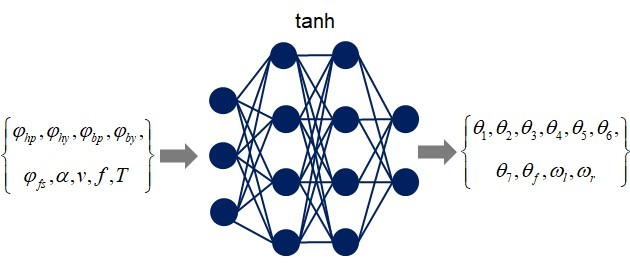
\includegraphics[width=0.8\textwidth]{network.jpg}
    \caption{Joint Trajectory learning by a two hidden-layer BP neural network.}
    \label{figure:Joint Trajectory learning by a two hidden-layer BP neural network}
\end{figure}

\subsection{Interaction Hypothesis}
Based on our robotic rat platform, we hope to learn the rat-like behavioral interaction by controlling the interaction process between two robots. Therefore, we put forward the following hypothesis: The interaction probability $P_{interaction}$ is affected by the centroid distance ($d_m$) and the average relative speed ($\nu_m$) between $\rm R_A$ and $\rm R_B$. We assumed that the smaller the centroid distance, or the larger the average relative speed between $\rm R_A$ and $\rm R_B$, the greater the probability of $\rm R_B$ executing the interaction pattern, as shown in the following formula:
\begin{equation} \label{eq:probability of interaciton}
    \displaystyle\begin{cases}
        u=\displaystyle\frac{\nu/V_m}{d_m/D_m} \\
        P_{interaciton}(u)=\displaystyle\frac{p_{+\infty}-p_{-\infty}}{1+e^{-ku}}+p_{-\infty}
    \end{cases}
\end{equation}

where $V_m$ and $D_m$ are the maximum values of average relative speed and centroid distance between $\rm R_A$ and $\rm R_B$, respectively, $-1\leq v_m/V_m\leq 1$ (the inner side of the centroid line is positive and the outer side is negative), $0\leq d_m/D_m\leq 1$ ($d_m>0$, because the defined interaciton process is noncontact). $p_{+\infty},p_{-\infty}$ and $k$ are interaction coefficients, which represent the lower limit, upper limit and scale factor of interaction probability $P_{interaciton}$, respectively, as shown in Figure. \ref{figure:relationship between the interaciton probability and independent variable}.
\begin{figure}[h]
    \centering
    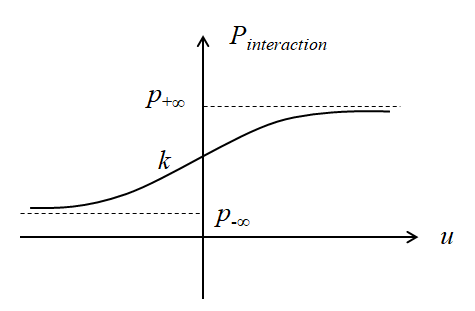
\includegraphics[width=0.8\textwidth]{interaction-probability.png}
    \caption{Relationship between the interaciton probability $P_{interaction}$ and independent variable $u$.}
    \label{figure:relationship between the interaciton probability and independent variable}
\end{figure}

In this paper, we used interaction information entropy to measure the interaction similarity between robots and rats \cite{lellis-feedback-control}, as shown in the following formula:
\begin{equation} \label{eq:interaction similarity}
    I(R_A,R_B)=\sum_{a_{i+1},b_i,b_{i+1}}p(a_{i+1},b_i,b_{i+1})\log_{2}\frac{p(b_{i+1}|a_{i+1}),b_{i}}{b_{i+1}|b_i}
\end{equation}
where $\rm R_A$ and $\rm R_B$ are the two rats or two robots that produce interaction. $I$ represents the amount of interaction information between two rats or two robots. The closer the amount of interaction information of robots is to the actual rats, the closer the interaction process of the two is. \textcolor{red}{$\Delta t~(t_i\rightarrow t_{i+1})$ is the movement duration $T_A$ of $\rm R_A$.}

\subsection{Robot Interactive Control}
In the interaction pattern, when $\rm R_A$ shows walking or trotting behavior, the state of $\rm R_B$ is tracking; when $\rm R_A$ shows other behaviors, the state of $\rm R_B$ is imitating. For the imitating state, the movement parameters of $\rm R_B$ are equal to those of $|rm R_A$. For the tracking state, as shown in Figure. \ref{figure:movement parameters of RB in the tracking state}. when the movement parameters of $\rm R_A$ are known, the movement parameters of $\rm R_B$ are as follows:
\begin{equation} \label{eq:movement parameters}
    \begin{cases}
        \nu_B=d_{m'}/T_A \\
        \alpha_B=\beta - \delta \\
        T_B=T_A
    \end{cases}
\end{equation}
\begin{figure}[h]
    \centering
    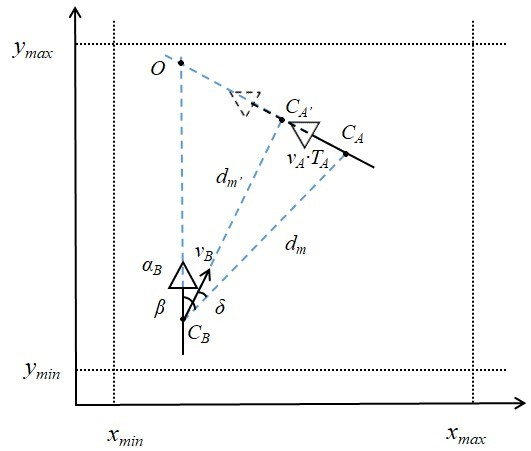
\includegraphics[width=0.8\textwidth]{movement parameters of rb.jpg}
    \caption{Movement parameters of $\rm R_B$ in the tracking state.}
    \label{figure:movement parameters of RB in the tracking state}
\end{figure}
$C_A,~C_{A'}$ and $C_B$ are the centroids of $\rm R_A$ at $t_i$ and $t_{i+1}$, and $\rm R_B$ at $t_{i+1}$ respectively.

In addition, we considered the problem of robot collision avoidance, as shown in Figure. \ref{figure:obstacle avoidance analysis}. Figure. \ref{figure:obstacle avoidance analysis}-\ref{figure:Avoid collision with boundary} shows the process of the robot avoiding collision with the boundary (wall). The condition of obstacle avoidance and the configuration of robot movement parameters are shown in Equation (\ref{eq:configuration of robot movement parameters}). Figure. \ref{figure:obstacle avoidance analysis}-\ref{figure:Avoid collision between robots} shows the process of avoiding collisions between robots. The condition for obstacle avoidance and the configuration of robot movement parameters are shown in Equation (\ref{eq:configuration2 of robot movement parameters}).

\begin{figure}[h]
    \centering
    \begin{subfigure}{0.4\textwidth}
        \centering
        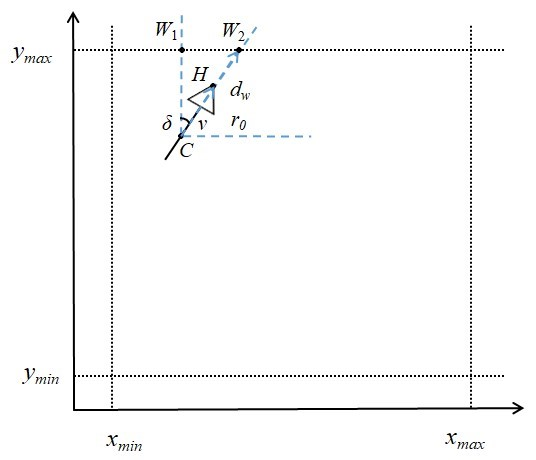
\includegraphics[height=2.2in]{collision-avoidance.jpg}
        \caption{\label{figure:Avoid collision with boundary}}
    \end{subfigure}
    \begin{subfigure}{0.4\textwidth}
        \centering
        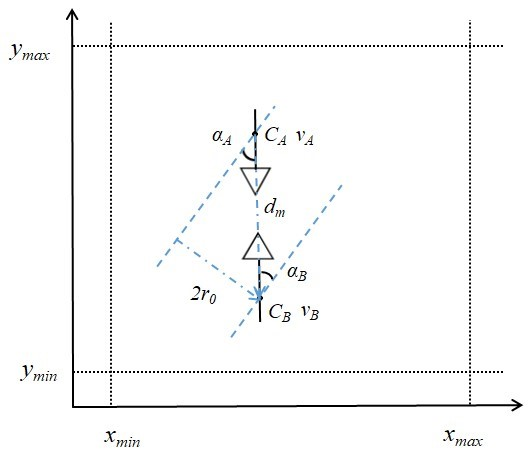
\includegraphics[height=2.2in]{collision-avoidance-between-robots.jpg}
        \caption{\label{figure:Avoid collision between robots}}
    \end{subfigure}
    \caption{Obstacle avoidance analysis. (\subref{figure:roboticrat}) Avoid collision with boundary (wall); (\subref{figure:motion-coord}) Avoid collision between robots.}
    \label{figure:obstacle avoidance analysis}
\end{figure}
\begin{equation}\label{eq:configuration of robot movement parameters}
    \begin{cases}
        d_w\leq D_w^{avoid} \\
        D_w^{avoid} = T_{control}\cdot \nu +r_0 \\
        \nu \rightarrow 0, \alpha=\pi/2-\delta, T_{control}
    \end{cases}
\end{equation}
\begin{equation}\label{eq:configuration2 of robot movement parameters}
    \begin{cases}
        d_m\leq D_m^{avoid} \\
        D_m^{avoid} = T_{control}\cdot \nu_m + 2r_0 \\
        \nu_A \rightarrow 0, \alpha_A, T_{control} \\
        \nu_B \rightarrow 0, \alpha_B, T_{control}
    \end{cases}
\end{equation}

\subsection{Hypothesis Test}
First, we observed the interaction process and calculated the interaction information entropy between rats ($I_{rat}=1.207$). Then, we gave a series of values of $p_{-\infty}, p_{+\infty}$ and $k$, and calculated the value of $I_{robot}$ in the interaciton time $T_{interaciton}$. $T_{interaciton}$ is the shortest time to make the interaction process converge. When the behavior probability distribution of the robot tends to be stable, we believe that the interaction process converges. Our results are shown in Table \ref{table:INTERACTION INFORMATION ENTROPY OF ROBOTS}.
\begin{table}[b]
    \caption{Interaction Information Entropy of Robots}
    \centering
    \begin{tabular}{ccccc}
            \hline
            $p_{-\infty}$ & $p_{+\infty}$ & $k$ & $I_{robot}$ & $\hat{I}_{robot}$\\
            \hline
            0.2 & 0.4 & 0.5 & 0.8987 & 0.9541 \\
            0.3 & 0.5 & 1 & 1.156 & 1.091 \\
            0.4 & 0.6 & 1.5 & 1.256 & 1.228 \\
            0.5 & 0.7 & 2 & 1.337 & 1.365 \\
            0.6 & 0.8 & 2.5 & 1.494 & 1.502 \\
            \hline
            \end{tabular}
    \label{table:INTERACTION INFORMATION ENTROPY OF ROBOTS}
\end{table}

After data analysis, we found that the independent variables have a significant impact on the dependent variable with a close linear correlation. Therefore, we used a multiple linear regression model to fit the relationship between independent variables and dependent variables, as shown in Equation (\ref{eq:multiple linear regression model}).
\begin{equation}\label{eq:multiple linear regression model}
    \hat{I}_{robot}=a_0+a_1p_{-\infty}+a_2p_{+\infty}+a_3k
\end{equation}
where the coefficients $a_i, i=0,1,2,3$ are calculated as follows ($n$ is the number of samples).
\begin{equation*}
    \left[\begin{array}{c}
        a_0 \\
        a_1 \\
        a_2 \\
        a_3 \\
    \end{array}\right]=\left[\begin{array}{cccc}
        n & \sum p_{-\infty} & \sum p_{+\infty}  & \sum k \\
        \sum p_{-\infty} & \sum p^2_{-\infty} & \sum p_{-\infty}p_{+\infty}  & \sum p_{-\infty} k \\
        \sum p_{+\infty} & \sum p_{-\infty} p_{+\infty} & \sum p^2_{+\infty}  & \sum p_{+\infty} k \\
        \sum k & \sum p_{-\infty} k & \sum p_{+\infty} k  & \sum k^2 \\
    \end{array}\right]^{-1}
    \left[\begin{array}{c}
        \sum I_{robot} \\
        \sum p_{-\infty} I_{robot} \\
        \sum p_{+\infty} I_{robot} \\
        \sum kI_{robot} \\
    \end{array}\right]
\end{equation*}
After calculation, we obtained $a_0=1.7282, a_1=0.1128, a_2=0.2584$, and $ a_3=0.0119$.

Furthermore, we obtained a set of control variables through parameter optimization, which makes the interaction information entropy of two robots and two rats closest. The Equation shows the process of parameter optimization, and the optimal solution is
\begin{equation}
    \begin{cases}
        p_{-\infty},p_{+\infty},k=\arg\min f \\
        \min f(p_{-\infty},p_{+\infty},k)=\displaystyle\frac{|I_{robot}-I_{rat}|}{I_{rat}} \\
        s.t.~0<p_{-\infty}<p_{+\infty}<1 \\
    \end{cases}
\end{equation}

We calculated the interaction information entropy between robots (10 times) by the optimal solution of control variables, and the results are shown in Table \ref{table:INTERACTION INFORMATION ENTROPY OF ROBOTS AND RATS}. The t-test shows that there is no significant difference between the interaction information entropy of two robots and two rats; that is, our hypothesis has been verified.
\begin{table}[b]
    \caption{Interaction Information Entropy of Robots and Rats}
    \centering
    \begin{tabular}{ccc}
            \hline
            $I_{robot}$ & ${I}_{rat}$ & t-test \\
            \hline
            1.210 &\multirow{9}{*}{1.207} & \multirow{9}{*}{$\begin{array}{l}
                H_0:\bar{I}_{robot}=I_{rat}; \\ H_1:\bar{I}_{robot}\neq I_{rat}; \\ t=1.583<t_{0.025,9}=2.262
            \end{array}$} \\
            1.108 & & \\
            1.208 & & \\
            1.206 & & \\
            1.207 & & \\
            1.211 & & \\
            1.207 & & \\
            1.205 & & \\
            1.205 & & \\
            \hline
            \end{tabular}
    \label{table:INTERACTION INFORMATION ENTROPY OF ROBOTS AND RATS}
\end{table}
